\documentclass[journal,12pt,twocolumn]{IEEEtran}

\usepackage{setspace}
\usepackage{gensymb}
\singlespacing
\usepackage[cmex10]{amsmath}

\usepackage{amsthm}

\usepackage{paralist}

\usepackage{mathrsfs}
\usepackage{txfonts}
\usepackage{stfloats}
\usepackage{bm}
\usepackage{cite}
\usepackage{cases}
\usepackage{subfig}

\usepackage{longtable}
\usepackage{multirow}
\usepackage{enumitem}
\usepackage{mathtools}
\usepackage{steinmetz}
\usepackage{tikz}
\usepackage{circuitikz}
\usepackage{verbatim}
\usepackage{tfrupee}
\usepackage[breaklinks=true]{hyperref}
\usepackage{graphicx}
\usepackage{tkz-euclide}

\usetikzlibrary{calc,math}
\usepackage{listings}
    \usepackage{color}                                            %%
    \usepackage{array}                                            %%
    \usepackage{longtable}                                        %%
    \usepackage{calc}                                             %%
    \usepackage{multirow}                                         %%
    \usepackage{hhline}                                           %%
    \usepackage{ifthen}                                           %%
    \usepackage{lscape}     
\usepackage{multicol}
\usepackage{chngcntr}

\DeclareMathOperator*{\Res}{Res}

\renewcommand\thesection{\arabic{section}}
\renewcommand\thesubsection{\thesection.\arabic{subsection}}
\renewcommand\thesubsubsection{\thesubsection.\arabic{subsubsection}}

\renewcommand\thesectiondis{\arabic{section}}
\renewcommand\thesubsectiondis{\thesectiondis.\arabic{subsection}}
\renewcommand\thesubsubsectiondis{\thesubsectiondis.\arabic{sub subsection}}


\hyphenation{optical networks semiconduc-tor}
\def\inputGnumericTable{}                                 %%

\lstset{
%language=C,
frame=single, 
breaklines=true,
columns=fullflexible
}
\date{March 2021}

\begin{document}

\newcommand{\BEQA}{\begin{eqnarray}}
\newcommand{\EEQA}{\end{eqnarray}}
\newcommand{\define}{\stackrel{\triangle}{=}}
\bibliographystyle{IEEEtran}
\raggedbottom
\setlength{\parindent}{0pt}
\providecommand{\mbf}{\mathbf}
\providecommand{\pr}[1]{\ensuremath{\Pr\left(#1\right)}}
\providecommand{\qfunc}[1]{\ensuremath{Q\left(#1\right)}}
\providecommand{\fn}[1]{\ensuremath{f\left(#1\right)}}
\providecommand{\e}[1]{\ensuremath{E\left(#1\right)}}
\providecommand{\sbrak}[1]{\ensuremath{{}\left[#1\right]}}
\providecommand{\lsbrak}[1]{\ensuremath{{}\left[#1\right.}}
\providecommand{\rsbrak}[1]{\ensuremath{{}\left.#1\right]}}
\providecommand{\brak}[1]{\ensuremath{\left(#1\right)}}
\providecommand{\lbrak}[1]{\ensuremath{\left(#1\right.}}
\providecommand{\rbrak}[1]{\ensuremath{\left.#1\right)}}
\providecommand{\cbrak}[1]{\ensuremath{\left\{#1\right\}}}
\providecommand{\lcbrak}[1]{\ensuremath{\left\{#1\right.}}
\providecommand{\rcbrak}[1]{\ensuremath{\left.#1\right\}}}
\theoremstyle{remark}
\newtheorem{rem}{Remark}
\newcommand{\sgn}{\mathop{\mathrm{sgn}}}
\providecommand{\abs}[1]{\vert#1\vert}
\providecommand{\res}[1]{\Res\displaylimits_{#1}} 
\providecommand{\norm}[1]{\lVert#1\rVert}
%\providecommand{\norm}[1]{\lVert#1\rVert}
\providecommand{\mtx}[1]{\mathbf{#1}}
\providecommand{\mean}[1]{E[ #1 ]}
\providecommand{\fourier}{\overset{\mathcal{F}}{ \rightleftharpoons}}
%\providecommand{\hilbert}{\overset{\mathcal{H}}{ \rightleftharpoons}}
\providecommand{\system}{\overset{\mathcal{H}}{ \longleftrightarrow}}
	%\newcommand{\solution}[2]{\textbf{Solution:}{#1}}
\newcommand{\solution}{\noindent \textbf{Solution: }}
\newcommand{\cosec}{\,\text{cosec}\,}
\providecommand{\dec}[2]{\ensuremath{\overset{#1}{\underset{#2}{\gtrless}}}}
\newcommand{\myvec}[1]{\ensuremath{\begin{pmatrix}#1\end{pmatrix}}}
\newcommand{\mydet}[1]{\ensuremath{\begin{vmatrix}#1\end{vmatrix}}}
\numberwithin{equation}{subsection}
\makeatletter
\vspace{3cm}
\title{Assignment 3}
\author{Adhvik Mani Sai Murarisetty - AI20BTECH11015}
\maketitle
\newpage
\bigskip
\renewcommand{\thetable}{\theenumi}
Download all python codes from 
\begin{lstlisting}
https://github.com/adhvik24/AI1103-PROBABILITY-AND-RANDOM-VARIABLES/tree/main/ASSIGNMENT_3/codes
\end{lstlisting}
%
and latex-tikz codes from 
%
\begin{lstlisting}
https://github.com/adhvik24/AI1103-PROBABILITY-AND-RANDOM-VARIABLES/blob/main/ASSIGNMENT_3/AI1103_Assignment3.tex
\end{lstlisting}
\section{Gate XE-A-2017-QN 2}
Three fair dies are rolled simultaneously. The probability of getting a sum of 5 is\\
\begin{inparaenum}[(A)]
    \item $\frac{1}{108}$\hspace{0.5cm}
    \item $\frac{1}{72}$\hspace{0.5cm}
    \item $\frac{1}{54}$\hspace{0.5cm}
    \item $\frac{1}{36}$
\end{inparaenum}

\section{Solution}
Let
$X_i\in\,$\cbrak{1,2,3,4,5,6}, i = 1,2,3, be the random variables representing the outcome for each die. As the dies are fair, the probability mass function (pmf) is expressed as
\begin{align}
    p_{X_i}(n) = \pr{X_i = n} = 
\begin{cases}
\frac{1}{6} & 1 \le n \le 6
\\
0 & otherwise
\end{cases}\label{1}
\end{align}
Let X be a random variable denotes the desired outcome,
\begin{align}
    X=X_1+X_2+X_3\label{2}\\
    \implies X\in\cbrak{3,4,\cdots,18}
\end{align}

We have to find $P_X(n)$ = $\pr{X_1+X_2+X_3=n}$
\begin{multline}
    p_X(n)=\pr{X_1+X_2+X_3=n}\\
   =\pr{X_1+X_2=n-X_3}\\
    =\Sigma_{k}{\pr{X_1+X_2=n-k|X_3=k}p_{X_3}(k)}\label{3}
\end{multline}
As $X_1,X_2,X_3$ are independent, After unconditioning
\begin{align}
    \pr{X_1+X_2=n-k|X_3=k}=\pr{X_1+X_2=n-k}\label{6}
\end{align}
Using \eqref{6} in \eqref{3}
\begin{multline}
    p_X(n)=\Sigma_{k}{\pr{X_1+X_2=n-k|X_3=k}p_{X_3}(k)}\\
    =\Sigma_{k}{\pr{X_1+X_2=n-k}p_{X_3}(k)}\\
    =\Sigma_{k}{\brak{\Sigma_{a}{\pr{X_1=n-k-a|X_2=a}\pr{X_2=a}}}p_{X_3}(k)}\\
    =\Sigma_{k}{\brak{\Sigma_{a}{\pr{X_1=n-k-a}\pr{X_2=a}}}p_{X_3}(k)}\\
    =\Sigma_{k}{\brak{\Sigma_{a}{p_{X_1}\brak{n-k-a}p_{X_2}\brak{a}}}p_{X_3}(k)}\label{4}
\end{multline}
Equation \eqref{4} can be written as follows using convolution operation,
\begin{align}
    \nonumber p_X(n)&=\Sigma_{k}{\brak{\Sigma_{a}{p_{X_1}\brak{n-k-a}p_{X_2}\brak{a}}}p_{X_3}(k)}\\
    &=p_{X_1}\brak{n}*p_{X_2}\brak{n}*p_{X_3}\brak{n}\label{5}
\end{align}
The Z-transform of $p_X(n)$ is defined as
\begin{align}
P_X(z) = \sum_{n = -\infty}^{\infty}p_X(n)z^{-n}, \quad z \in \mathbb{C}
\label{7}
\end{align}
%
From \eqref{1} and \eqref{7}, 
\begin{align}
\nonumber P_{X_1}(z) =P_{X_2}(z)&=P_{X_3}(z)\\
&= \frac{1}{6}\sum_{n = 1}^{6}z^{-n}
\\
&=\frac{z^{-1}\brak{1-z^{-6}}}{6\brak{1-z^{-1}}}, \quad \abs{z} > 1
\label{8}
\end{align}
upon summing up the geometric progression. 
From \eqref{5},
\begin{align}
\because p_X(n) &= p_{X_1}(n)*p_{X_2}(n)*p_{X-3}(n),
\\
P_X(z) &= P_{X_1}(z) P_{X_2}(z)P_{X_3}(z)
\label{9}
\end{align}
The above property follows from Fourier analysis and is fundamental to signal processing.\\
From \eqref{8} and \eqref{9},
\begin{align}
    P_X{\brak{z}}&=\cbrak{\frac{z^{-1}\brak{1-z^{-6}}}{6\brak{1-z^{-1}}}}^3\\
    &= \frac{1}{216}\frac{z^{-3}\brak{1-3z^{-6}+3z^{-12}-z^{-18}}}{\brak{1-z^{-1}}^3}\label{10}
\end{align}
Using the fact that,
\begin{align}
p_X(n-k) &\system{Z}P_X(z)z^{-k},
\\
nu(n)&\system{Z} \frac{z^{-1}}{\brak{1-z^{-1}}^2}\\
n^2u(n)&\system{Z} \frac{z^{-1}\brak{1+z^{-1}}}{\brak{1-z^{-1}}^3}\\
(n^2+n)u(n)&\system{Z} \frac{2z^{-1}}{\brak{1-z^{-1}}^2}
\end{align}
after some algebra, it can be shown that,
\begin{multline}
\frac{1}{216\times 2}\lsbrak{\brak{(n-2)^2+n-2}u(n-2)} \\-3 \brak{(n-8)^2+n-8}u(n-8)\\+3\brak{(n-14)^2+n-14}u(n-14)\\-\rsbrak{\brak{(n-20)^2+n-20}u(n-20)}
\\
\system{Z}
\frac{1}{216}\frac{z^{-3}\brak{1-3z^{-6}+3z^{-12}-z^{-18}}}{\brak{1-z^{-1}}^3}
\label{11}
\end{multline}
where 
\begin{align}
u(n) =
\begin{cases}
1 & n \ge 0
\\
0 & n < 0\label{13}
\end{cases}
\end{align}
From \eqref{7},\eqref{10} and \eqref{11},
\begin{multline}
p_{X}(n) = \frac{1}{216\times 2}\lsbrak{\brak{(n-2)^2+n-2}u(n-2)} \\-3 \brak{(n-8)^2+n-8}u(n-8)\\+3\brak{(n-14)^2+n-14}u(n-14)\\-\rsbrak{\brak{(n-20)^2+n-20}u(n-20)}
\label{12}
\end{multline}
From \eqref{13} and \eqref{12},
\begin{align}
p_X(n) &= 
\begin{cases}
0 & n < 3\\
\frac{n^2-3n+2}{432} &  3 \le n \le  8\\
\frac{42n-2n^2-166}{432} & 8 < n \le 14\\
\frac{n^2-39n+380}{432} & 14 < n \le 18\\
0 & n > 18\label{14}
\end{cases}
\end{align}
\begin{figure}[htp]
    \centering
    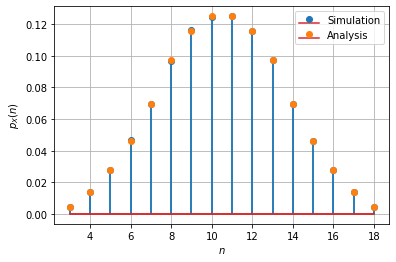
\includegraphics[width=\columnwidth]{assign3_stem.png}
    \caption{Probability mass function of X}{ (simulations are close to analysis)}
\end{figure}
We need probability of getting sum of 5,\\$\implies$ n=5 \\from \eqref{14} and using n=5,
\begin{align}
    p_X(5)&=\frac{5^2-3(5)+2}{432}\\
    p_X(5)&=\frac{12}{432}\\
    p_X(5)&=\frac{1}{36}
\end{align}
\begin{figure}[htp]
    \centering
    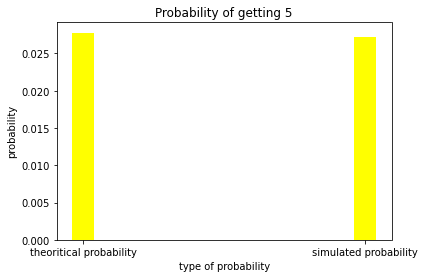
\includegraphics[width=\columnwidth]{assign3.png}
    \caption{Probability of getting sum of 5}
\end{figure}

Therefore the probability of getting a sum of 5 when three fair dies are rolled is $\frac{1}{36}$.\\
\textbf{Ans: Option (D)}
\end{document}
